%%%%%%%%%%%%%%%%%%%%%%%%%%%%%%%%%%%%%%%%%%%%%%%%%%%%%%%%%%%%%%%%%%%%%%
% LaTeX Template: Curriculum Vitae
%
% Source: http://www.howtotex.com/
% Feel free to distribute this template, but please keep the
% referal to HowToTeX.com.
% Date: July 2011
% 
%%%%%%%%%%%%%%%%%%%%%%%%%%%%%%%%%%%%%%%%%%%%%%%%%%%%%%%%%%%%%%%%%%%%%%
% How to use writeLaTeX: 
%
% You edit the source code here on the left, and the preview on the
% right shows you the result within a few seconds.
%
% Bookmark this page and share the URL with your co-authors. They can
% edit at the same time!
%
% You can upload figures, bibliographies, custom classes and
% styles using the files menu.
%
% If you're new to LaTeX, the wikibook is a great place to start:
% http://en.wikibooks.org/wiki/LaTeX
%
%%%%%%%%%%%%%%%%%%%%%%%%%%%%%%%%%%%%%%%%%%%%%%%%%%%%%%%%%%%%%%%%%%%%%%
\documentclass[paper=a4,fontsize=11pt]{scrartcl} % KOMA-article class
							
\usepackage[english]{babel}
\usepackage[utf8x]{inputenc}
\usepackage[protrusion=true,expansion=true]{microtype}
\usepackage{amsmath,amsfonts,amsthm}     % Math packages
\usepackage{graphicx}                    % Enable pdflatex
\usepackage[svgnames]{xcolor}            % Colors by their 'svgnames'
\usepackage{geometry}
	\textheight=700px                    % Saving trees ;-)
\usepackage{url}
\usepackage{siunitx}

\frenchspacing              % Better looking spacings after periods
\pagestyle{empty}           % No pagenumbers/headers/footers

%%% Custom sectioning (sectsty package)
%%% ------------------------------------------------------------
\usepackage{sectsty}

\sectionfont{%			            % Change font of \section command
	\usefont{OT1}{phv}{b}{n}%		% bch-b-n: CharterBT-Bold font
	\sectionrule{0pt}{0pt}{-5pt}{3pt}}

%%% Macros
%%% ------------------------------------------------------------
\newlength{\spacebox}
\settowidth{\spacebox}{8888888888}			% Box to align text
\newcommand{\sepspace}{\vspace*{1em}}		% Vertical space macro

\newcommand{\MyName}[1]{ % Name
		\Huge \usefont{OT1}{phv}{b}{n} \hfill #1
		\par \normalsize \normalfont}
		
\newcommand{\MySlogan}[1]{ % Slogan (optional)
		\large \usefont{OT1}{phv}{m}{n}\hfill \textit{#1}
		\par \normalsize \normalfont}

\newcommand{\NewPart}[1]{\section*{\uppercase{#1}}}

\newcommand{\PersonalEntry}[2]{
		\noindent\hangindent=2em\hangafter=0 % Indentation
		\parbox{\spacebox}{        % Box to align text
		\textit{#1}}		       % Entry name (birth, address, etc.)
		\hspace{1.5em} #2 \par}    % Entry value

\newcommand{\SkillsEntry}[2]{      % Same as \PersonalEntry
		\noindent\hangindent=2em\hangafter=0 % Indentation
		\parbox{\spacebox}{        % Box to align text
		\textit{#1}}			   % Entry name (birth, address, etc.)
		\hspace{1.5em} #2 \par}    % Entry value	
		
\newcommand{\EducationEntry}[4]{
		\noindent \textbf{#1} \hfill      % Study
		\colorbox{Black}{%
			\parbox{6em}{%
			\hfill\color{White}#2}} \par  % Duration
		\noindent \textit{#3} \par        % School
		\noindent\hangindent=2em\hangafter=0 \small #4 % Description
		\normalsize \par}

\newcommand{\WorkEntry}[4]{				  % Same as \EducationEntry
		\noindent \textbf{#1} \hfill      % Jobname
		\colorbox{Black}{\color{White}#2} \par  % Duration
		\noindent \textit{#3} \par              % Company
		\noindent\hangindent=2em\hangafter=0 \small #4 % Description
		\normalsize \par}

%%% Begin Document
%%% ------------------------------------------------------------
\begin{document}
% you can upload a photo and include it here...
%\begin{wrapfigure}{l}{0.5\textwidth}
%	\vspace*{-2em}
%		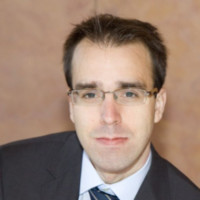
\includegraphics[width=0.15\textwidth]{photo}
%\end{wrapfigure}

\MyName{Genti Saliu}
\MySlogan{Curriculum Vitae}

\sepspace

%%% Personal details
%%% ------------------------------------------------------------
\NewPart{Personal details}{}

\PersonalEntry{Birth}{July 15, 1985}
\PersonalEntry{Address}{Hammäcker 13, 76189 Karlsruhe, Germany}
\PersonalEntry{Phone}{+49 157 3627 6029}
\PersonalEntry{Mail}{\url{gentisaliu@gmail.com}}
\PersonalEntry{Nationality}{Albanian}

%%% Education
%%% ------------------------------------------------------------
\NewPart{Education}{}

\EducationEntry{BSc. Physics}{2012 - 2018}{Karlsruhe Institute of Technology}{
\begin{itemize}
    \item Minor in Computer Science: Basic Notions of Computer Science I, Microcomputers Laboratory Courses and Algorithms I
    \item Additional courses in Advanced Mathematics, seminar on Collaborative Software Design for Physicists
    \item Seminar on Mössbauer spectroscopy
    \item Bachelor thesis on the improvement of $s$-channel single top quark reconstruction at a center-of-mass energy of \SI{13}{TeV} with the CMS experiment using an artifical neural-network classifier
\end{itemize}}
\sepspace

\EducationEntry{Diplom Computer Science (Did Not Graduate)}{2005 - 2008}{Karlsruhe Institute of Technology}{
\begin{itemize}
    \item Completed courses on Algorithm Design, Formal Languages, Introduction to the Java Programming Language, Numerical Analysis, Introduction to Probability Theory and Statistics
    \item Lab on System Architecture: implementation of various thread scheduling strategies and of the ’‘Battleship’‘ game with a UI and a network layer for multiplayer support
\end{itemize}}
\sepspace

%%% Work experience
%%% ------------------------------------------------------------
\NewPart{Work experience}{}

\WorkEntry{Full-Stack Software Developer}{Mar 2016 - Jul 2018}{Green Parrot GmbH, Working Student}{\begin{itemize}
    \item Developed backend (ASP.NET MVC, C\#, MongoDB, Redis) and frontend (KnockoutJS, AngularJS 1.x) features for the company’s main product: a price comparison search engine for buses, trains and car-shares
    \item DevOps tasks using Kubernetes, Google Cloud Engine and bare-metal server (Windows Server, Linux) management and implementation of server hardening processes
    \item Ported the support forum to Google Cloud Engine with Kubernetes: autoscaled \emph{nginx} and \emph{php-fpm} independently by creating two deployments and services respectively that share data via a volume running on a network-based file system
    \item Implemented features for similar acquired websites by the company in Romania and Bulgaria (PHP), and various internal company dashboards (VueJS, AngularJS)
    \item Built command-line utilities (C\#) for internal use
    \item Wrote technical documentation
\end{itemize}}
\sepspace

\WorkEntry{Student Software Developer}{Oct 2012 - Feb 2016}{Fraunhofer IOSB, Student Assistant}{
\begin{itemize}
    \item Attended a 2-day seminar on ''Methods of agile software development''
    \item Represented Fraunhofer IOSB at the CeBIT 2014 fair on March 12 - 14, 2014 demonstrating tools developed for the \emph{EO2Heaven} project
\end{itemize}

\emph{TRIDEC} (Tsunami Early Warning System)
\begin{itemize}
    \item Developed a web-based tool for the visualization of tweets related to tsunamis and earthquakes and of the results of their linguistic analysis (JavaScript, REST calls)
    \item Developed a web-based editor of business rules that generates and deploys Drools decision tables into a knowledge repository running on Activiti (Python, Django)
    \item Co-developed a linguistic and location analysis tool for Twitter text messages (Java) 
    \item Wrote software documentation
\end{itemize}
\sepspace
\emph{EO2Heaven} (Earth Observation and Environmental Modelling for the Mitigation of Health Risks)
\begin{itemize}
    \item Developed a web-based tool for interactive cholera outbreak visualization in Uganda (LeafletJS, WebGenesis CMS REST APIs)
\end{itemize}
\sepspace
\emph{StanDAP-Herb} (System for mass digitalization of herbarium labels)
\begin{itemize}
    \item Developed a single page application for OCR quality assurance and implement REST API endpoints for handling data
    \item Tested integration of a Drools-based decision table in an Activiti-run BPMN process
    \item Implemented SOAP web services in C\#.NET
\end{itemize}
\sepspace
\emph{IDEAM}
\begin{itemize}
    \item Developed a command-line tool for parsing disease data from Excel files (PHP)
    \item Developed a web-based tool for visualizing disease outbreak (LeafletJS, MarionetteJS, BackboneJS, SCSS, Bower, Gulp)
\end{itemize}}
\sepspace

\WorkEntry{Software Developer}{May 2011 - Sep 2015}{ICT Technologies UG, Working Student}{
\begin{itemize}
    \item Planned and developed a component-based object oriented PHP web development framework for a tennis portal (MyTennisDate) consisting of a database abstraction layer, autoloading, templating system, session handling, event system, security (input escaping, XSS and database injection prevention), utility functions for creating multi-step wizards, reusable views with logic, and asset management among others.
    \item Developed several eCommerce systems (B2C) using PHP, Symfony2, ExtJS, RequireJS, BackboneJS and MarionetteJS
    \item Developed continuous integration solutions in bare metal servers consisting of shell scripts and code repository integrations
\end{itemize}}
\sepspace

\WorkEntry{Full-Stack Developer}{Oct 2009 - Apr 2010}{eyeworkers Interactive GmbH, Working Student}{
\begin{itemize}
    \item Implemented customer-specific software customizations using jQuery, ExtJS, PHP (company websites, intranet-based web application for management of patient files for the Diaconate Hospital Karlsruhe-Rüppurr) and the company's own content management system, eyekit
    \item Performed on-site customer support
\end{itemize}}
\sepspace

\WorkEntry{Frontend Developer}{Jul 2009 - Aug 2009}{1\&1 Internet SE, Working Student}{
\begin{itemize}
    \item Deployed and integrated the acquired Jimdo content management system in the company's systems
    \item Developed WYSIWYG modules for Jimdo
\end{itemize}}
\sepspace

\WorkEntry{Software Developer}{Dec 2008 - Aug 2009}{B-ITE GmbH, Remote Developer}{Implemented backend and frontend features for a human resource management SaaS using MySQL, PHP, jQuery and jQuery plugins}
\sepspace

\WorkEntry{Software Developer}{Aug 2008 - Oct 2008}{Scanpoint Deutschland GmbH, Working Student}{Developed an intranet web application for tracking digitalized documents and OCR errors using JBoss, JavaServer Pages, JavaServer Faces and JasperReports}
\sepspace

\WorkEntry{Software Developer}{Mar 2008 - Dec 2014}{Freelancer}{
\begin{itemize}
    \item Development of plugins and customizations for the Zen Cart online store management and the Joomla content management system
    \item Third-party integrations of APIs (payments, data providers and consumers)
    \item Development of other custom software (details upon request)
\end{itemize}}

%%% Skills
%%% ------------------------------------------------------------
\NewPart{Skills}{}

\SkillsEntry{Languages}{Albanian (native language)}
\SkillsEntry{}{English (full professional proficiency)}
\SkillsEntry{}{German (full professional proficiency)}
\SkillsEntry{}{Italian (limited professional proficiency)}
\vspace{5mm}
\SkillsEntry{Software}{\textsc{Mathematica}, \LaTeX, \textsc{ROOT}, \textsc{Eclipse}}
\SkillsEntry{}{\textsc{Visual Studio}, \textsc{JetBrains Rider}, \textsc{JetBrains PHPStorm}}
\vspace{5mm}
\SkillsEntry{Programming}{\textsc{Java}, \textsc{C++}, \textsc{C\#}, \textsc{PHP}, \textsc{Haskell}, \textsc{Python}}
\SkillsEntry{Web}{Django with Python, Symfony and Laravel with PHP}
\SkillsEntry{}{ASP.NET Core, JavaServerPages, JavaServer Faces}
\SkillsEntry{Map APIs}{LeafletJS, GeoServer, Google Maps API, OpenLayers}
\SkillsEntry{GUI}{WinForms, Windows Presentation Foundation, Qt}
\SkillsEntry{AI}{Keras with Tensorflow}
\SkillsEntry{Databases}{\textsc{MySQL}, \textsc{Redis}, \textsc{MongoDB}}
\SkillsEntry{DevOps}{Kubernetes, Docker, Google Cloud Engine}

%%% References
%%% ------------------------------------------------------------
\NewPart{References}{}
Available upon request
\end{document}
